\FloatBarrier
\begin{figure*}[!t]
\centering
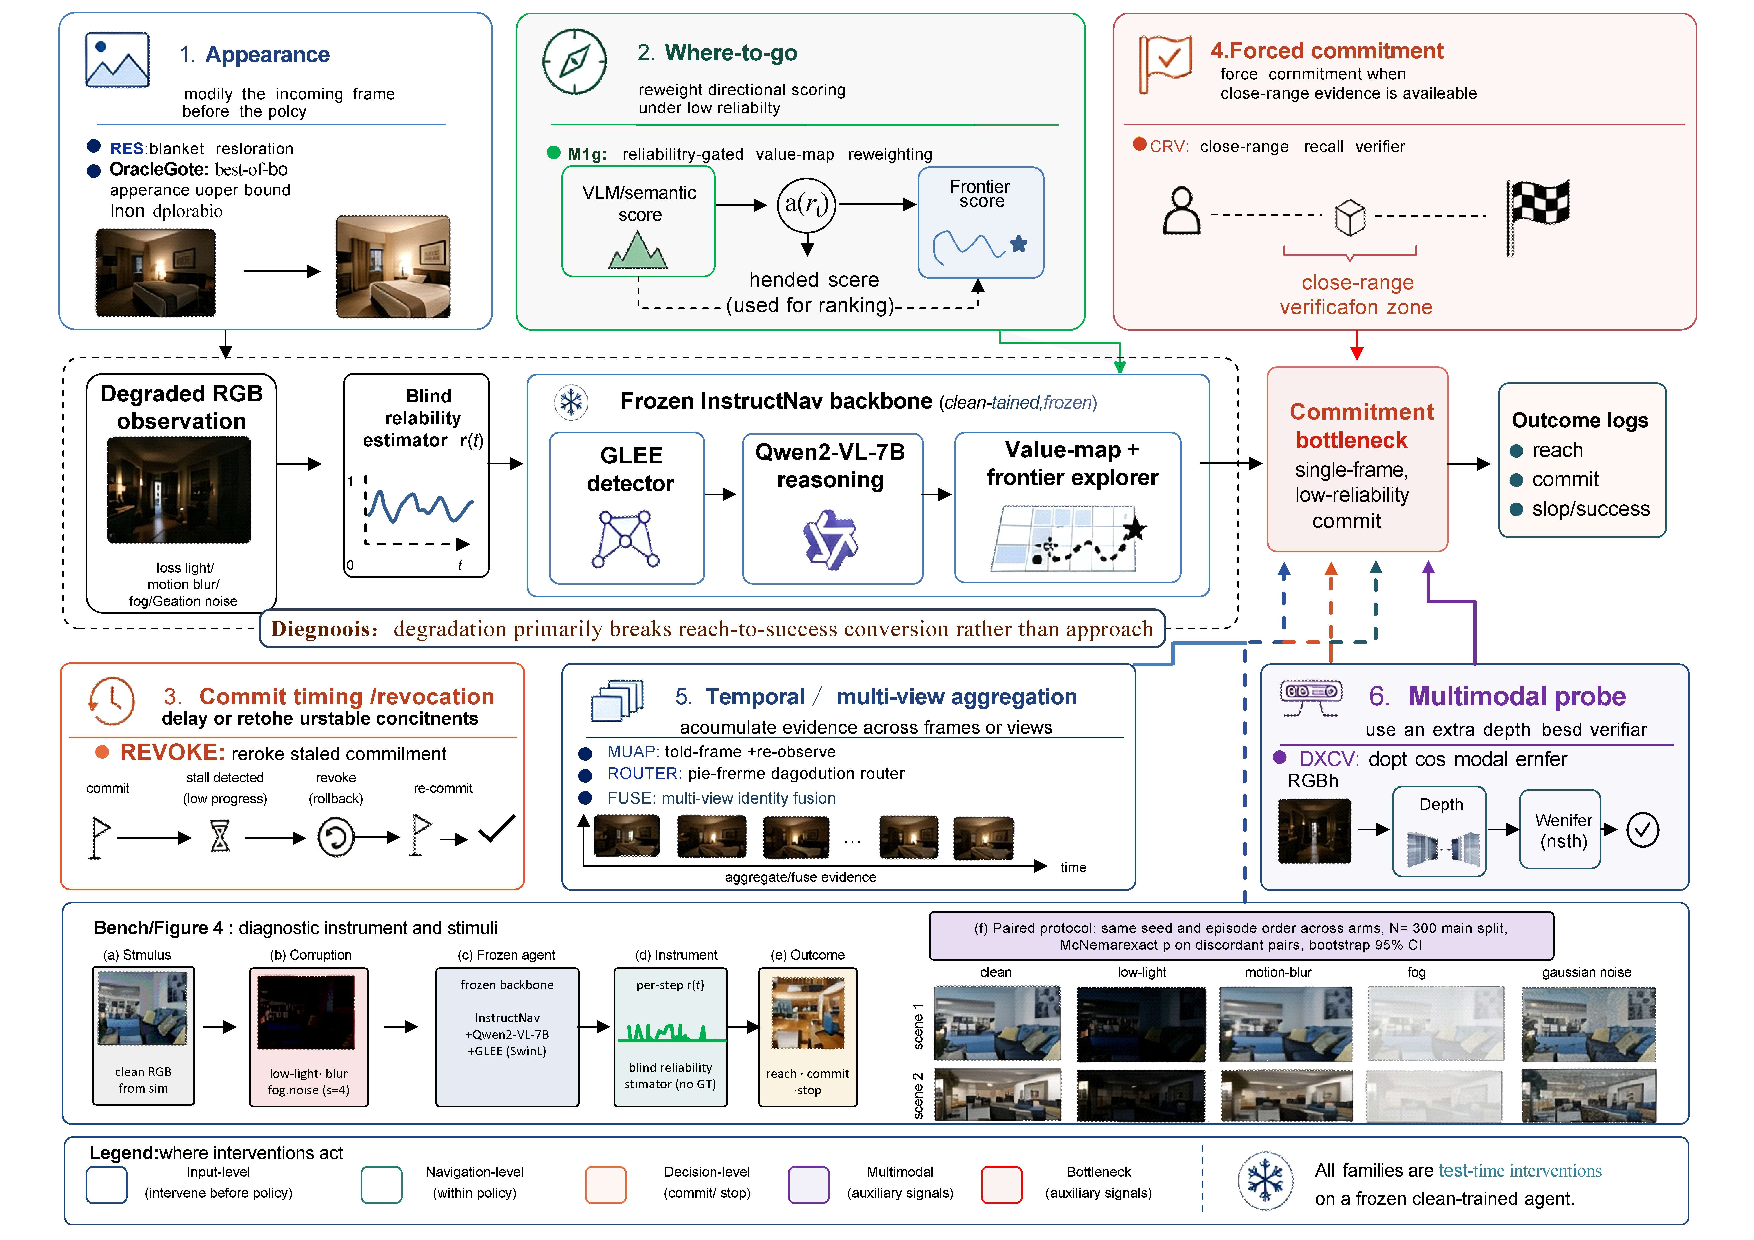
\includegraphics[width=0.88\textwidth]{figures/method.pdf}
\caption{
\textbf{From diagnosis to candidate interventions.}
A degraded RGB observation is passed through a blind per-step
reliability estimator and a frozen InstructNav backbone (GLEE,
Qwen2-VL-7B, and a value-map frontier explorer), whose outcome logs
localize failure to a \emph{commitment bottleneck}
(Sec.~\ref{sec:motivation}): degradation primarily breaks
reach-to-success conversion rather than approach.
The six surrounding panels instantiate the intervention families tested
in this paper: \textbf{(1)} appearance modification (RES, OracleGate),
\textbf{(2)} reliability-gated where-to-go reweighting,
\textbf{(3)} commit timing / revocation,
\textbf{(4)} forced commitment,
\textbf{(5)} temporal / multi-view aggregation, and
\textbf{(6)} a depth-based multimodal probe.
The bottom strip summarizes the benchmark substrate and paired protocol:
structure-preserving corruptions, a frozen clean-trained backbone, and
same-seed same-episode paired comparisons with McNemar exact tests and
bootstrap $95\%$ CIs.
}
\label{fig:method}
\end{figure*}

\section{Related Work}

\paragraph{Zero-shot object navigation with foundation models.}
Object-goal navigation \citep{batra2020objectnav} and vision-and-language
navigation \citep{anderson2018r2r,krantz2020vlnce,khanna2024goat} are
typically learned with reinforcement or imitation \citep{wijmans2020ddppo,
ramrakhya2023pirlnav}, which generalizes poorly to unseen distributions.
Zero-shot systems instead build on foundation models. One family
guides frontier exploration with language priors
\citep{chaplot2020semexp,zhou2023esc,yu2023l3mvn}; another fuses
open-vocabulary detectors into a value map for goal reasoning
\citep{yokoyama2024vlfm,gadre2023cow}; a third lets a VLM read a panoramic
observation and emit a heading \citep{zhou2024navgpt,
long2024instructnav}. We build on InstructNav \citep{long2024instructnav},
an agent that couples a VLM, an open-vocabulary detector
\citep{wu2024glee}, and a value-map frontier explorer. These works assume
clean observations; we instead study, on the same backbone, \emph{where}
such an agent breaks when its input is degraded.

\paragraph{Robustness of embodied agents to visual corruption.}
RobustNav \citep{chattopadhyay2021robustnav} first benchmarked navigation
under visual and dynamics corruptions and reported large drops, motivating
task-oriented data augmentation \citep{maksymets2021thda} and domain
adaptation. A common alternative is to restore the input before it reaches
the policy via low-light enhancement \citep{guo2020zerodce,wu2023uretinex}
or denoising, which operate at the pixel layer and aim to recover clean
appearance. We show that, for a VLM-driven navigator, restoring appearance
does not restore navigation: an $8.4$\,dB PSNR gain leaves SR within seed
noise, and a per-frame oracle that always picks the better-looking view
does no better. Our benchmark exposes this gap, with a paired protocol and
severity sweeps in the style of corruption robustness benchmarks
\citep{hendrycks2019benchmarking}.

\paragraph{Uncertainty, commitment, and executive control.}
Knowing when a model should not be trusted is central to safe autonomy
\citep{abdar2021uncertainty}; blind image-quality assessment estimates
degradation without a reference \citep{su2020blindly} and active perception
decides where to look to reduce uncertainty
\citep{ramakrishnan2021exploration}. A complementary direction studies the
\emph{executive} layer of zero-shot ObjectNav: \emph{when} to commit, stop,
and recover. We use a training-free per-step reliability estimate purely as
a \emph{measurement instrument}, and evaluate deployable commitment-timing
and temporal/multi-view aggregation interventions head-on; each leaves
success unchanged or lowers it on a frozen, clean-trained backbone
(Table~\ref{tab:sweep}).

\begin{figure*}[!t]
\centering
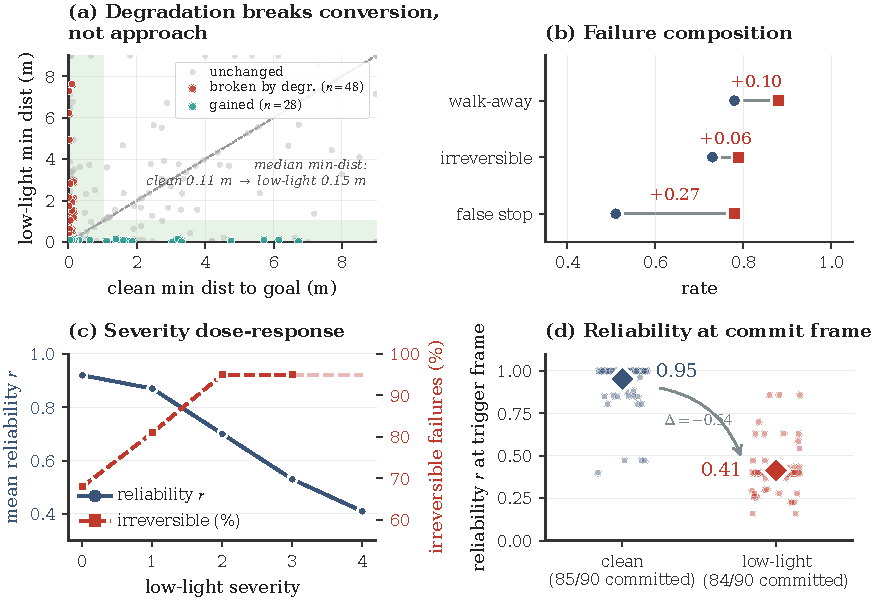
\includegraphics[width=0.88\textwidth]{figures/fig_motivation.pdf}
\caption{\textbf{Method-independent motivation study (baseline InstructNav).}
\textbf{(a)}~Paired min-distance, clean vs.\ low-light severity~$4$ (same
$300$ episodes): approach geometry barely moves (median $0.11\to0.15$\,m)
yet $48$ episodes flip to failure---degradation breaks \emph{conversion},
not approach. \textbf{(b)}~M2 ($n{=}90$): failures shift toward walk-aways
and irreversible failures. \textbf{(c)}~M3: severity lowers reliability;
the irreversible fraction saturates. \textbf{(d)}~M4: the deciding
commitment fires on a single low-$r$ frame (mean $0.95{\to}0.41$).}
\label{fig:motivation}
\end{figure*}